\documentclass[11pt,letterpaper]{article}

% CODIFICACIÓN E IDIOMA
\usepackage[utf8]{inputenc}     
\usepackage[T1]{fontenc}         % Salida de fuentes en T1: acentos y guionado correctos
\usepackage[spanish]{babel}      % Localización: "Tabla", "Figura", "Demostración", fechas, etc.
\decimalpoint
\usepackage{microtype}           % Micro-ajustes tipográficos (mejora notable de legibilidad)

% MATEMÁTICAS

\usepackage{amsmath,amssymb,amsfonts,amsthm}
\usepackage{mathtools}
\providecommand{\abs}[1]{\lvert#1\rvert}
\providecommand{\norm}[1]{\lVert#1\rVert}
\newcommand{\Aut}{\operatorname{Aut}}

% TIPOGRAFÍA

\usepackage{newpxtext,newpxmath}
\usepackage{titlesec}            % Formato de \section, \subsection, etc.

% GEOMETRÍA DE PÁGINA
\usepackage[a4paper,letterpaper,margin=2.5cm,headheight=14.5pt,includeheadfoot]{geometry}



% FIGURAS, TABLAS Y CÓDIGO

\usepackage{graphicx}
\graphicspath{{imagenes/}{figuras/}{img/}}
\usepackage{subcaption}          % Sustituye a "subfigure" (paquete obsoleto desde 2001)
\usepackage{caption}
\captionsetup{font=small,labelfont=bf,margin=8pt}
\usepackage{booktabs}            % Tablas profesionales (\toprule, \midrule, \bottomrule)
\usepackage{array}
\usepackage{siunitx}
% \sisetup{output-decimal-marker = {.}, group-separator = {,}}
% \sisetup{
%     locale = US,
%     output-decimal-marker = {.},
%     group-separator = {,}
% }
\usepackage{enumitem}            % Listas con espaciado controlado
\usepackage{listings}
\usepackage{xcolor}
\usepackage{tikz}
\usepackage{pgfplots}
\pgfplotsset{compat=1.18}        % Versión de compatibilidad actualizada (1.15 → 1.18)
\usetikzlibrary{arrows.meta}     % Sustituye a la librería "arrows", ya obsoleta


% ESPACIADO DE PÁRRAFOS
\setlength{\parindent}{0pt}
\setlength{\parskip}{0.65em plus 0.1em minus 0.1em}


% HIPERVÍNCULOS (se carga casi al final, como recomienda su documentación)
\usepackage{hyperref}
\hypersetup{
    colorlinks   = true,
    linkcolor    = {primary},
    citecolor    = {primary},
    urlcolor     = {primary!70!black},
    pdfborder    = {0 0 0},
    breaklinks   = true,
    bookmarksnumbered = true
}


% PALETA DE COLORES

\definecolor{primary}{RGB}{120,25,90}    % Vino/púrpura institucional (evolución de "purpura")
\definecolor{secondary}{RGB}{70,70,70}   % Gris oscuro para texto secundario
\definecolor{bgcode}{RGB}{247,247,250}   % Fondo suave para bloques de código
\hypersetup{linkcolor=primary, citecolor=primary, urlcolor=primary!70!black}

% TÍTULOS DE SECCIÓN 

\titleformat{\section}
  {\normalfont\Large\bfseries\sffamily\color{primary}}
  {\thesection}{0.8em}{}[{\color{primary!60}\titlerule[0.8pt]}]
\titlespacing*{\section}{0pt}{2.8ex plus 1ex minus .2ex}{1.4ex plus .2ex}

\titleformat{\subsection}
  {\normalfont\large\bfseries\sffamily\color{primary!85!black}}
  {\thesubsection}{0.8em}{}
\titlespacing*{\subsection}{0pt}{2.2ex plus 1ex minus .2ex}{1ex plus .2ex}

\titleformat{\subsubsection}
  {\normalfont\normalsize\bfseries\sffamily\color{secondary}}
  {\thesubsubsection}{0.8em}{}


% ENCABEZADO Y PIE DE PÁGINA

\usepackage{fancyhdr}
\pagestyle{fancy}
\fancyhf{}
\renewcommand{\headrulewidth}{0.6pt}
\renewcommand{\footrulewidth}{0.4pt}
\fancyheadoffset{0pt}

% Estilo "plain" (usado en la portada) sin encabezado
\fancypagestyle{plain}{%
  \fancyhf{}
  \renewcommand{\headrulewidth}{0pt}
  \renewcommand{\footrulewidth}{0pt}
}

% Datos del documento 
\newcommand{\asignaturaNombre}{Matemáticas}
\newcommand{\tareaNombre}{Tarea 2}
\newcommand{\autorNombre}{Eduardo Alanís García}
\newcommand{\institucionNombre}{MCDI}
\newcommand{\profesorNombre}{Dra. Briceyda B. Delgado López}
\newcommand{\fechaEntrega}{26 de septiembre de 2026}


\fancyhead[L]{\small\color{primary}\textbf{\asignaturaNombre}}
\fancyhead[R]{\small\color{primary}\textbf{\tareaNombre}}
\fancyfoot[L]{\small\color{secondary}\autorNombre}
\fancyfoot[C]{\small\color{secondary}\thepage}
\fancyfoot[R]{\small\color{secondary}\institucionNombre}


% ENTORNOS TIPO TEOREMA
\newtheoremstyle{coloredplain}
  {0.9em}{0.9em}{\normalfont}{0pt}{\bfseries\color{primary}}{.}{0.6em}{}
\newtheoremstyle{coloreddef}
  {0.9em}{0.9em}{\normalfont}{0pt}{\bfseries\color{primary!75!black}}{.}{0.6em}{}

\theoremstyle{coloredplain}
\newtheorem{teorema}{Teorema}[section]
\newtheorem{lema}[teorema]{Lema}
\newtheorem{proposicion}[teorema]{Proposición}
\newtheorem{corolario}[teorema]{Corolario}

\theoremstyle{coloreddef}
\newtheorem{definicion}{Definición}[section]
\newtheorem{ejemplo}[definicion]{Ejemplo}
\newtheorem{observacion}[definicion]{Nota}
\newtheorem{afirmacion}[definicion]{Afirmación}
\newtheorem{pregunta}[definicion]{Pregunta}
\newtheorem{respuesta}[definicion]{Respuesta}
\newtheorem{ejercicio}{Ejercicio}


\renewcommand{\qedsymbol}{$\blacksquare$}
\newenvironment{solucion}
  {\par\noindent\textbf{\color{primary}Solución.}\ }
  %{\hfill$\blacksquare$\par}

\newenvironment{demostraccion}
  {\par\noindent\textbf{\color{primary}Demostración.}\ }
  {\hfill$\blacksquare$\par}

\newcommand{\pie}[1]{\footnote{#1}}


% CÓDIGO FUENTE (bloques "listings" con estilo unificado)

\lstdefinestyle{Rstyle}{
    language        = R,
    backgroundcolor = \color{bgcode},
    basicstyle      = \ttfamily\small,
    keywordstyle    = \color{primary}\bfseries,
    commentstyle    = \color{secondary}\itshape,
    stringstyle     = \color{teal},
    numbers         = left,
    numberstyle     = \tiny\color{secondary},
    numbersep       = 8pt,
    frame           = single,
    rulecolor       = \color{primary!30},
    breaklines      = true,
    showstringspaces= false,
    captionpos      = b,
    tabsize         = 2
}
\lstset{style=Rstyle}


% Referencias
\usepackage{csquotes}
\usepackage[numbers]{natbib}
% ============================================================================


% ============================================================================
\begin{document}


% PORTADA

\begin{titlepage}
  \thispagestyle{plain}
  \centering
  \vspace*{2.5cm}

  {\sffamily\color{secondary}\large Maestría en Ciencia de Datos e Información \par}
  \vspace{0.3cm}
  {\color{primary}\rule{0.5\textwidth}{0.8pt}\par}
  \vspace{2.2cm}

  {\sffamily\bfseries\color{primary}\Huge \tareaNombre \par}
  \vspace{0.6cm}
  {\sffamily\Large \asignaturaNombre \par}

  \vspace{3.5cm}
  {\color{primary!60}\rule{0.6\textwidth}{0.4pt}\par}
  \vspace{1cm}

  \begin{tabular}{rl}
    \textbf{Alumno:}   & \autorNombre \\[2pt]
    \textbf{Profesora:} & \profesorNombre \\[2pt]
    \textbf{Entrega:}    & \fechaEntrega \\
  \end{tabular}

  \vfill
  {\small\color{secondary} INFOTEC \par}
\end{titlepage}

% Descomente si desea un índice automático:
% \tableofcontents
% \newpage


\section*{Instrucciones}
Lea el archivo \emph{Formato de tareas} que se encuentra en la siguiente liga
\url{https://drive.google.com/drive/u/0/folders/1F-FI1J5PviBc-EPhfLbnE8PSvWnkgeHj}.

En la siguiente lista de ejercicios NO se admite ningún tipo de código en la
solución de los ejercicios, cada uno de ellos se puede resolver de forma
analítica. La única excepción es el ejercicio 5, donde se indica sea resuelto
usando el paquete R. Párrafos que contengan código en la entrega no se van a
considerar en la calificación.

\section*{Ejercicios}

% EJERCICIO 1

\begin{ejercicio}[15 puntos]
  La función de densidad de una variable aleatoria está dada por
  \[
    f(x) =
    \begin{cases}
      a + bx^{2}, & 0 \leq x \leq 1,\\
      0, & \text{en otro caso.}
    \end{cases}
  \]
  Si la esperanza es $E(X) = \dfrac{3}{5}$. Encuentre $a$ y $b$.

  
\begin{solucion}
    Por definicion de función de densidad \citep{rincon2014prob} cumple que 
    \[
      \int_{-\infty}^{\infty} f(x)\,dx = 1
    \]
    Como $f(x)=0$ fuera del intervalo $[0,1]$, tenemos
    \[
      \int_{0}^{1} (a+bx^{2})\,dx = 1
    \]
    Entonces:
    \[
      \int_{0}^{1} (a+bx^{2})\,dx
      = \left[ax+\frac{b}{3}x^{3}\right]_{0}^{1}
      = a+\frac{b}{3}.
    \]
    Por lo tanto
    \[
      a+\frac{b}{3}=1
    \]
 
    Por otro lado, por definición, la esperanza de una
    variable aleatoria continua \citetext{\citealp[Sección~2.6]{rincon2014prob}; \citealp{notasclase}} es
    \[
      E(X)=\int_{-\infty}^{\infty} x\,f(x)\,dx.
    \]
    De esta manera:
    \[
      E(X)=\int_{0}^{1} x(a+bx^{2})\,dx
      =\int_{0}^{1} (ax+bx^{3})\,dx
      =\left[\frac{a}{2}x^{2}+\frac{b}{4}x^{4}\right]_{0}^{1}
      =\frac{a}{2}+\frac{b}{4}
    \]
    Como se nos indica que $E(X)=\dfrac{3}{5}$, obtenemos 
    \[
      \frac{a}{2}+\frac{b}{4}=\frac{3}{5}
    \]
 
    Obteniendo el sistema
    \[
      \begin{cases}
        a+\dfrac{1}{3}b=1 \\[0.5em]
        \dfrac{1}{2}a+\dfrac{1}{4}b=\dfrac{3}{5}
      \end{cases}
    \]
    Resolvemos por Gauss-Jordan
    \[
    \begin{aligned}
    \left[
    \begin{array}{cc|c}
    1 & \frac{1}{3} & 1\\
    \frac{1}{2} & \frac{1}{4} & \frac{3}{5}
    \end{array}
    \right]
    &\xrightarrow{R_2\leftarrow R_2-\frac{1}{2}R_1}
    \left[
    \begin{array}{cc|c}
    1 & \frac{1}{3} & 1\\
    0 & \frac{1}{12} & \frac{1}{10}
    \end{array}
    \right]
    &\xrightarrow{R_2\leftarrow 12R_2}
    \left[
    \begin{array}{cc|c}
    1 & \frac{1}{3} & 1\\
    0 & 1 & \frac{6}{5}
    \end{array}
    \right]
    \xrightarrow{R_1\leftarrow R_1-\frac{1}{3}R_2}
    \left[
    \begin{array}{cc|c}
    1 & 0 & \frac{3}{5}\\
    0 & 1 & \frac{6}{5}
    \end{array}
    \right]
    \end{aligned}
    \]
 
    Por lo tanto,
    \[
      a=\frac{3}{5},\qquad b=\frac{6}{5}
    \]
 
    \textbf{Verificación.} Tenemos que $f(x)=\dfrac{3}{5}+\dfrac{6}{5}x^{2}$
    en $[0,1]$, que es no negativa en todo el intervalo, verificamos las dos condiciones:
    \[
      \int_{0}^{1}\left(\frac{3}{5}+\frac{6}{5}x^{2}\right)dx
      = \frac{3}{5}+\frac{6}{5}\cdot\frac{1}{3}
      = \frac{3}{5}+\frac{2}{5}=1, 
    \]
    \[
      \int_{0}^{1} x\left(\frac{3}{5}+\frac{6}{5}x^{2}\right)dx
      = \frac{3}{10}+\frac{6}{5}\cdot\frac{1}{4}
      = \frac{3}{10}+\frac{3}{10}=\frac{6}{10}=\frac{3}{5}
    \]
    Ambas condiciones se satisfacen, por lo que los valores $a=\dfrac{3}{5}$
    y $b=\dfrac{6}{5}$ son correctos.
  \end{solucion}
\end{ejercicio}
 
 
% EJERCICIO 2
 
\begin{ejercicio}[10 puntos]
  La estatura de las mujeres adultas en Estados Unidos se distribuye
  normalmente con media de $\mu = 64.5$ pulgadas y desviación estándar de
  $\sigma = 2.4$ pulgadas. Hallar la probabilidad de que una mujer elegida al
  azar mida
  \begin{enumerate}[label=(\alph*)]
    \item Mida menos de 63 pulgadas;
    \item Mida entre 63 y 70 pulgadas.
    \item Alice mide 72 pulgadas. ¿Qué porcentaje de mujeres mide menos que
      Alicia?
  \end{enumerate}
 
  \begin{solucion}
    Sea $X$ la variable aleatoria que representa la estatura (en pulgadas)
    de una mujer adulta elegida al azar en Estados Unidos. Por el enunciado,
    $X\sim N(\mu,\sigma^{2})$ con
    \[
      \mu=64.5,\qquad \sigma=2.4.
    \]
    Para calcular cualquier probabilidad usamos la estandarización \citep[Sección~3.13]{rincon2014prob}
    \[
      Z=\frac{X-\mu}{\sigma}\ \sim\ N(0,1)
    \]
    y consultamos el valor correspondiente en la tabla de la distribución
    normal estándar, $\Phi(z)=P(Z\leq z)$ \citep[Sección~3.13]{rincon2014prob}.
 
    \begin{enumerate}[label=(\alph*)]
 
      \item \textbf{$P(X<63)$.} Estandarizamos el valor $x=63$:
      \[
        z=\frac{63-\mu}{\sigma}=\frac{63-64.5}{2.4}=\frac{-1.5}{2.4}=-0.625
      \]
      Buscamos $\Phi(-0.625)$. Usando la simetría de la normal estándar,
      $\Phi(-z)=1-\Phi(z)$, así que basta encontrar $\Phi(0.625)$. En la
      tabla, los valores más cercanos son
      \[
        \Phi(0.62) = 0.73237,\qquad \Phi(0.63) = 0.73565
      \]
      De esta manera para $z=0.625$ (punto medio entre ambos)
      obtenemos
      \[
        \Phi(0.625)\approx \frac{0.73237+0.73565}{2}= 0.73401 \approx 0.7340
      \]
      Por lo tanto,
      \[
        P(X<63)=\Phi(-0.625)=1-\Phi(0.625)\approx 1-0.7340=0.2660
      \]
      Es decir, la probabilidad de que una mujer elegida al azar mida menos
      de $63$ pulgadas es de aproximadamente $0.2660$, es decir, un
      $26.60 \%$.
 
      \item \textbf{$P(63<X<70)$.} Ya tenemos $z$ para $x=63$ del inciso
      anterior. Estandarizamos ahora $x=70$:
      \[
        z=\frac{70-\mu}{\sigma}=\frac{70-64.5}{2.4}=\frac{5.5}{2.4}\approx
        2.29
      \]
      Buscamos en la tabla $\Phi(2.29)=  0.98899 \approx0.9890$.
 
      Como la probabilidad de que $X$ esté entre dos valores es la
      diferencia de las probabilidades acumuladas hasta cada uno de ellos \citep[Sección~2.3]{rincon2014prob}
      \[
        P(63<X<70)=P(X<70)-P(X<63)=\Phi(2.29)-\Phi(-0.625)
      \]
      De esta manera
      \[
        P(63<X<70)\approx 0.9890-0.2660=0.7230.
      \]
      Por lo tanto, la probabilidad de que una mujer elegida al azar mida
      entre $63$ y $70$ pulgadas es de aproximadamente $0.7230$, es
      decir, un $72.30 \%$.
 
      \item Porcentaje de mujeres que miden menos que Alice
      ($x=72$). Estandarizamos $x=72$:
      \[
        z=\frac{72-\mu}{\sigma}=\frac{72-64.5}{2.4}=\frac{7.5}{2.4}=3.125
      \]
      De esta manera
      \[
        P(X<72)=\Phi(3.125)\approx 0.9991.
      \]
      Esto significa que aproximadamente el $99.91 \%$ de las
      mujeres miden menos que Alice; es decir, solo alrededor del
      $0.09 \%$ de las mujeres son tan altas como ella o más altas. 
    \end{enumerate}
  \end{solucion}
\end{ejercicio}
 


% EJERCICIO 3

\begin{ejercicio}[25 puntos]
  Realice un análisis de las temperaturas promedio de uno de los 32 estados
  de México de los años 1993 al 2023 aproximando a través del método de
  mínimos cuadrados para el caso lineal, cuadrático y cúbico. El caso lineal
  y cuadrático se explicaron en clase, para en caso cúbico es necesario
  utilizar el mismo razonamiento y deducir las fórmulas resultantes. Explicar
      paso a paso el método.

  Los estados y el periodo se asignarán de forma personalizada, véase el
  final del archivo. Los datos provienen del Servicio Metereológico
  Nacional\footnote{\url{https://smn.conagua.gob.mx/es/8-smn-general}} De
  click en la pestaña Climatología, seguido de Temperaturas y Lluvia, luego
  seleccione la opción Resúmenes mensuales de Temperaturas y Lluvia.


  Estado asignado: \textbf{Aguascalientes}  
\end{ejercicio}


\begin{solucion}
    Deduciremos primero la fórmula correspondiente al caso cúbico, siguiendo el mismo razonamiento empleado en clase para los casos lineal y cuadrático \citep{notasclase}.

    Consideremos una función cúbica
    \[
      p(t) = \alpha + \beta t + \gamma t^{2} + \theta t^{3}
    \]
    que minimice la suma de los errores cuadrados. El problema consiste entonces en resolver
    \[
      \min_{\alpha,\ \beta,\ \gamma,\ \theta}\ \sum_{i=1}^{n} \left( \alpha + \beta t_i + \gamma t_i^{2} + \theta t_i^{3} - y_i \right)^{2}.
    \]

    Definimos la función
    \[
      F(\alpha, \beta, \gamma, \theta) = \sum_{i=1}^{n} \left( \alpha + \beta t_i + \gamma t_i^{2} + \theta t_i^{3} - y_i \right)^{2}.
    \]

    Para minimizar $F$ respecto a las variables $\alpha, \beta, \gamma$ y $\theta$, las condiciones necesarias son
    \[
      \frac{\partial F}{\partial \alpha}
      = \frac{\partial F}{\partial \beta}
      = \frac{\partial F}{\partial \gamma}
      = \frac{\partial F}{\partial \theta}
      = 0.
    \]

    Calculamos cada una de estas derivadas parciales.

    Derivada respecto a $\alpha$.
    \[
      \frac{\partial F}{\partial \alpha}
      = 2\sum_{i=1}^{n} \left( \alpha + \beta t_i + \gamma t_i^{2} + \theta t_i^{3} - y_i \right) = 0
      \iff
      \alpha\, n + \beta \sum_{i=1}^{n} t_i + \gamma \sum_{i=1}^{n} t_i^{2} + \theta \sum_{i=1}^{n} t_i^{3} = \sum_{i=1}^{n} y_i.
    \]

    Derivada respecto a $\beta$.
    \[
      \frac{\partial F}{\partial \beta}
      = 2\sum_{i=1}^{n} \left( \alpha + \beta t_i + \gamma t_i^{2} + \theta t_i^{3} - y_i \right) t_i = 0
      \iff
      \alpha \sum_{i=1}^{n} t_i + \beta \sum_{i=1}^{n} t_i^{2} + \gamma \sum_{i=1}^{n} t_i^{3} + \theta \sum_{i=1}^{n} t_i^{4} = \sum_{i=1}^{n} y_i t_i.
    \]

    Derivada respecto a $\gamma$.
    \[
      \frac{\partial F}{\partial \gamma}
      = 2\sum_{i=1}^{n} \left( \alpha + \beta t_i + \gamma t_i^{2} + \theta t_i^{3} - y_i \right) t_i^{2} = 0
      \iff
      \alpha \sum_{i=1}^{n} t_i^{2} + \beta \sum_{i=1}^{n} t_i^{3} + \gamma \sum_{i=1}^{n} t_i^{4} + \theta \sum_{i=1}^{n} t_i^{5} = \sum_{i=1}^{n} y_i t_i^{2}.
    \]

    Derivada respecto a $\theta$.
    \[
      \frac{\partial F}{\partial \theta}
      = 2\sum_{i=1}^{n} \left( \alpha + \beta t_i + \gamma t_i^{2} + \theta t_i^{3} - y_i \right) t_i^{3} = 0
      \iff
      \alpha \sum_{i=1}^{n} t_i^{3} + \beta \sum_{i=1}^{n} t_i^{4} + \gamma \sum_{i=1}^{n} t_i^{5} + \theta \sum_{i=1}^{n} t_i^{6} = \sum_{i=1}^{n} y_i t_i^{3}.
    \]

    De esta manera, obtenemos el siguiente sistema de ecuaciones
    \begin{align*}
      \alpha\, n + \beta \sum_{i=1}^{n} t_i + \gamma \sum_{i=1}^{n} t_i^{2} + \theta \sum_{i=1}^{n} t_i^{3} &= \sum_{i=1}^{n} y_i, \\
      \alpha \sum_{i=1}^{n} t_i + \beta \sum_{i=1}^{n} t_i^{2} + \gamma \sum_{i=1}^{n} t_i^{3} + \theta \sum_{i=1}^{n} t_i^{4} &= \sum_{i=1}^{n} y_i t_i, \\
      \alpha \sum_{i=1}^{n} t_i^{2} + \beta \sum_{i=1}^{n} t_i^{3} + \gamma \sum_{i=1}^{n} t_i^{4} + \theta \sum_{i=1}^{n} t_i^{5} &= \sum_{i=1}^{n} y_i t_i^{2}, \\
      \alpha \sum_{i=1}^{n} t_i^{3} + \beta \sum_{i=1}^{n} t_i^{4} + \gamma \sum_{i=1}^{n} t_i^{5} + \theta \sum_{i=1}^{n} t_i^{6} &= \sum_{i=1}^{n} y_i t_i^{3}. 
    \end{align*}

    El cual podemos reescribir en forma matricial como sigue. 
    \[
      \begin{pmatrix}
        n & \displaystyle\sum_{i=1}^{n} t_i & \displaystyle\sum_{i=1}^{n} t_i^{2} & \displaystyle\sum_{i=1}^{n} t_i^{3} \\[1em]
        \displaystyle\sum_{i=1}^{n} t_i & \displaystyle\sum_{i=1}^{n} t_i^{2} & \displaystyle\sum_{i=1}^{n} t_i^{3} & \displaystyle\sum_{i=1}^{n} t_i^{4} \\[1em]
        \displaystyle\sum_{i=1}^{n} t_i^{2} & \displaystyle\sum_{i=1}^{n} t_i^{3} & \displaystyle\sum_{i=1}^{n} t_i^{4} & \displaystyle\sum_{i=1}^{n} t_i^{5} \\[1em]
        \displaystyle\sum_{i=1}^{n} t_i^{3} & \displaystyle\sum_{i=1}^{n} t_i^{4} & \displaystyle\sum_{i=1}^{n} t_i^{5} & \displaystyle\sum_{i=1}^{n} t_i^{6}
      \end{pmatrix}
      \begin{pmatrix}
        \alpha \\ \beta \\ \gamma \\ \theta
      \end{pmatrix}
      =
      \begin{pmatrix}
        \displaystyle\sum_{i=1}^{n} y_i \\[1em]
        \displaystyle\sum_{i=1}^{n} y_i t_i \\[1em]
        \displaystyle\sum_{i=1}^{n} y_i t_i^{2} \\[1em]
        \displaystyle\sum_{i=1}^{n} y_i t_i^{3}
      \end{pmatrix}.
    \]

    Por lo tanto, los coeficientes de la función cubica buscada son

    \[
      \begin{pmatrix}
        \alpha \\ \beta \\ \gamma \\ \theta
      \end{pmatrix}
      =
      \begin{pmatrix}
        n & \displaystyle\sum_{i=1}^{n} t_i & \displaystyle\sum_{i=1}^{n} t_i^{2} & \displaystyle\sum_{i=1}^{n} t_i^{3} \\[1em]
        \displaystyle\sum_{i=1}^{n} t_i & \displaystyle\sum_{i=1}^{n} t_i^{2} & \displaystyle\sum_{i=1}^{n} t_i^{3} & \displaystyle\sum_{i=1}^{n} t_i^{4} \\[1em]
        \displaystyle\sum_{i=1}^{n} t_i^{2} & \displaystyle\sum_{i=1}^{n} t_i^{3} & \displaystyle\sum_{i=1}^{n} t_i^{4} & \displaystyle\sum_{i=1}^{n} t_i^{5} \\[1em]
        \displaystyle\sum_{i=1}^{n} t_i^{3} & \displaystyle\sum_{i=1}^{n} t_i^{4} & \displaystyle\sum_{i=1}^{n} t_i^{5} & \displaystyle\sum_{i=1}^{n} t_i^{6}
      \end{pmatrix}^{-1}
      \begin{pmatrix}
        \displaystyle\sum_{i=1}^{n} y_i \\[1em]
        \displaystyle\sum_{i=1}^{n} y_i t_i \\[1em]
        \displaystyle\sum_{i=1}^{n} y_i t_i^{2} \\[1em]
        \displaystyle\sum_{i=1}^{n} y_i t_i^{3}
      \end{pmatrix}
    \]

\textbf{Herramientas y datos.} Los promedios anuales se obtuvieron de los resúmenes mensuales del Servicio Meteorológico Nacional. Las sumas y la gráfica se calcularon con R. El procedimiento completo y los datos están disponibles en: \href{https://eduardo-alanis-garcia.github.io/MCDI_1er_Semestre/Matematicas/Unidad\%202.\%20Probabilidad/code/E3/Minimos\%20Cuadrados\%20R.html}{Mínimos Cuadrados R (Eduardo Alanís García)}.

Aplicaremos ahora el método de mínimos cuadrados a los datos de temperatura, usando el caso lineal y el cuadrático (vistos en clase \citep{notasclase}) y el caso cúbico (deducido arriba).


Para ello consideramos los años con la variable $t_i = i$, $i = 1, \dots, 31$,
de modo que $t_1 = 1$ corresponde a 1993 y $t_{31} = 31$ corresponde a 2023;
$y_i$ denota la temperatura promedio del $i$-ésimo año. 

\begin{center}
\captionof{table}{Temperatura media anual de Aguascalientes, 1993--2023.}
\label{tab:aguascalientes}
\begin{minipage}{0.4\textwidth}
\centering
\begin{tabular}{ccc}
\hline
Año & $t_i$ & $y_i$ ($^\circ$C) \\
\hline
1993 & 1 & 17.5 \\
1994 & 2 & 17.7 \\
1995 & 3 & 17.6 \\
1996 & 4 & 17.4 \\
1997 & 5 & 17.4 \\
1998 & 6 & 17.6 \\
1999 & 7 & 17.6 \\
2000 & 8 & 17.7 \\
2001 & 9 & 18.0 \\
2002 & 10 & 18.0 \\
2003 & 11 & 17.2 \\
2004 & 12 & 17.1 \\
2005 & 13 & 17.7 \\
2006 & 14 & 17.9 \\
2007 & 15 & 17.7 \\
2008 & 16 & 17.9 \\
\hline
\end{tabular}
\end{minipage}
\hspace{1cm}
\begin{minipage}{0.4\textwidth}
\centering
\begin{tabular}{ccc}
\hline
Año & $t_i$ & $y_i$ ($^\circ$C) \\
\hline
2009 & 17 & 17.8 \\
2010 & 18 & 17.8 \\
2011 & 19 & 18.0 \\
2012 & 20 & 17.9 \\
2013 & 21 & 17.9 \\
2014 & 22 & 17.5 \\
2015 & 23 & 17.6 \\
2016 & 24 & 17.4 \\
2017 & 25 & 17.9 \\
2018 & 26 & 17.8 \\
2019 & 27 & 18.4 \\
2020 & 28 & 18.1 \\
2021 & 29 & 17.4 \\
2022 & 30 & 17.9 \\
2023 & 31 & 18.7 \\
\hline
\end{tabular}
\end{minipage}
\end{center}


Con $n = 31$ datos se
obtienen

\[
\sum_{i=1}^{31} t_i = 496, \quad
\sum_{i=1}^{31} t_i^{2} = 10416, \quad
\sum_{i=1}^{31} t_i^{3} = 246016, \quad
\sum_{i=1}^{31} t_i^{4} = 6\,197\,520,
\]
\[
\sum_{i=1}^{31} t_i^{5} = 162\,616\,576, \qquad
\sum_{i=1}^{31} t_i^{6} = 4\,388\,434\,896,
\]
\[
\sum_{i=1}^{31} y_i = 550.1, \qquad
\sum_{i=1}^{31} y_i t_i = 8843.2, \qquad
\sum_{i=1}^{31} y_i t_i^{2} = 186259.6, \qquad
\sum_{i=1}^{31} y_i t_i^{3} = 4\,408\,958.8.
\]

Con estos valores resolvemos los tres sistemas normales.

\subsubsection*{Caso lineal}

El sistema para $p_1(t) = \alpha + \beta t$ el sistema es
\[
\begin{pmatrix}
n & \sum t_i \\
\sum t_i & \sum t_i^{2}
\end{pmatrix}
\begin{pmatrix} \alpha \\ \beta \end{pmatrix}
=
\begin{pmatrix} \sum y_i \\ \sum y_i t_i \end{pmatrix}.
\]

Sustituyendo,
\[
\begin{pmatrix} \alpha \\ \beta \end{pmatrix}
=
\begin{pmatrix} 31 & 496 \\ 496 & 10416 \end{pmatrix}^{-1}
\begin{pmatrix} 550.1 \\ 8843.2 \end{pmatrix}
=
\begin{pmatrix}
\dfrac{21}{155} & -\dfrac{1}{155} \\[0.6em]
-\dfrac{1}{155} & \dfrac{1}{2480}
\end{pmatrix}
\begin{pmatrix} 550.1 \\ 8843.2 \end{pmatrix}
\approx
\begin{pmatrix} 17.47677419 \\ 0.01677419 \end{pmatrix}.
\]

De modo que la aproximación lineal es
\[
p_1(t) \approx 17.47677419 + 0.01677419\, t.
\]

\subsubsection*{Caso cuadrático}

Para $p_2(t) = \alpha + \beta t + \gamma t^{2}$, el sistema es
\[
\begin{pmatrix}
n & \sum t_i & \sum t_i^{2} \\
\sum t_i & \sum t_i^{2} & \sum t_i^{3} \\
\sum t_i^{2} & \sum t_i^{3} & \sum t_i^{4}
\end{pmatrix}
\begin{pmatrix} \alpha \\ \beta \\ \gamma \end{pmatrix}
=
\begin{pmatrix} \sum y_i \\ \sum y_i t_i \\ \sum y_i t_i^{2} \end{pmatrix}.
\]

Sustituyendo,
\[
\begin{pmatrix} \alpha \\ \beta \\ \gamma \end{pmatrix}
=
\begin{pmatrix}
31 & 496 & 10416 \\
496 & 10416 & 246016 \\
10416 & 246016 & 6\,197\,520
\end{pmatrix}^{-1}
\begin{pmatrix} 550.1 \\ 8843.2 \\ 186259.6 \end{pmatrix}
=
\begin{pmatrix}
\dfrac{1489}{4495} & -\dfrac{189}{4495} & \dfrac{1}{899} \\[0.6em]
-\dfrac{189}{4495} & \dfrac{5439}{791120} & -\dfrac{2}{9889} \\[0.6em]
\dfrac{1}{899} & -\dfrac{2}{9889} & \dfrac{1}{158224}
\end{pmatrix}
\begin{pmatrix} 550.1 \\ 8843.2 \\ 186259.6 \end{pmatrix}
\approx
\begin{pmatrix} 17.58222470 \\ -0.00239862 \\ 0.00059915 \end{pmatrix}.
\]

Así, la aproximación cuadrática es
\[
p_2(t) \approx 17.58222470 - 0.00239862\, t + 0.00059915\, t^{2}.
\]

\subsubsection*{Caso cúbico}

Usando el sistema $4\times 4$ deducido al inicio para
$p_3(t) = \alpha + \beta t + \gamma t^{2} + \theta t^{3}$, sustituimos los
valores numéricos:
\[
\begin{pmatrix} \alpha \\ \beta \\ \gamma \\ \theta \end{pmatrix}
=
\begin{pmatrix}
31 & 496 & 10416 & 246016 \\
496 & 10416 & 246016 & 6\,197\,520 \\
10416 & 246016 & 6\,197\,520 & 162\,616\,576 \\
246016 & 6\,197\,520 & 162\,616\,576 & 4\,388\,434\,896
\end{pmatrix}^{-1}
\begin{pmatrix} 550.1 \\ 8843.2 \\ 186259.6 \\ 4\,408\,958.8 \end{pmatrix}
\]
\[
=
\begin{pmatrix}
\dfrac{597}{899} & -\dfrac{851}{5394} & \dfrac{9}{899} & -\dfrac{1}{5394} \\[0.6em]
-\dfrac{851}{5394} & \dfrac{78655}{1\,669\,536} & -\dfrac{3325}{1\,008\,678} & \dfrac{3121}{48\,416\,544} \\[0.6em]
\dfrac{9}{899} & -\dfrac{3325}{1\,008\,678} & \dfrac{657}{2\,689\,808} & -\dfrac{5}{1\,008\,678} \\[0.6em]
-\dfrac{1}{5394} & \dfrac{3121}{48\,416\,544} & -\dfrac{5}{1\,008\,678} & \dfrac{5}{48\,416\,544}
\end{pmatrix}
\begin{pmatrix} 550.1 \\ 8843.2 \\ 186259.6 \\ 4\,408\,958.8 \end{pmatrix}
\approx
\begin{pmatrix} 17.41835373 \\ 0.05458013 \\ -0.00378243 \\ 0.00009128 \end{pmatrix}.
\]

Por lo que la aproximación cúbica es
\[
p_3(t) \approx 17.41835373 + 0.05458013\, t - 0.00378243\, t^{2} + 0.00009128\, t^{3}.
\]

\subsubsection*{Resultados}

Las tres aproximaciones por mínimos cuadrados para la temperatura promedio
anual de Aguascalientes, son:
\[
p_1(t) \approx 17.47677 + 0.01677\, t,
\]
\[
p_2(t) \approx 17.58222 - 0.00240\, t + 0.00060\, t^{2},
\]
\[
p_3(t) \approx 17.41835 + 0.05458\, t - 0.00378\, t^{2} + 0.00009\, t^{3}.
\]

Evaluando en los extremos del periodo se obtiene:

\begin{center}
\begin{tabular}{lccc}
 & $p_1(t)$ & $p_2(t)$ & $p_3(t)$ \\
\hline
$t=1$ (1993) & $17.4935\ ^\circ$C & $17.5804\ ^\circ$C & $17.4692\ ^\circ$C \\
$t=31$ (2023) & $17.9968\ ^\circ$C & $18.0837\ ^\circ$C & $18.1948\ ^\circ$C \\
\end{tabular}
\end{center}

Ademas las graficas compartiva es
\begin{center}
    \includegraphics[width=1\textwidth]{Tarea 2 Grafica Minimo Cuadrados}
\end{center}


Los tres polinomios señalan un aumento de la temperatura
media anual de Aguascalientes entre 1993 y 2023: los modelos lineal y cuadrático
estiman un incremento de $\approx 0.5\,^\circ$C y el cúbico de
$\approx 0.7\,^\circ$C. Dentro del periodo 1993--2023 los tres polinomios
prácticamente coinciden, ya que la diferencia máxima entre el modelo lineal y el
cúbico es de $\approx 0.2\,^\circ$C (en $t=31$), y entre el lineal y el
cuadrático de $\approx 0.09\,^\circ$C. Los términos adicionales solo agregan una
curvatura leve, menor que la variación de año a año que muestran los datos. Por
simplicidad, el modelo lineal es suficiente para describir la tendencia: indica
un aumento de $\approx 0.017\,^\circ$C por año, es decir, unos $0.17\,^\circ$C
por década.

Además, notemos que los puntos se dispersan alrededor de
las tres curvas, por lo que los modelos describen la tendencia general y no los
valores de cada año. Asimismo, estos modelos solo son válidos para el periodo
1993--2023.


    
\end{solucion}


% EJERCICIO 4

\begin{ejercicio}[10 puntos]
  El cáncer de próstata es el más frecuente entre los varones. Como
  indicador de si un varón padece cáncer de próstata, los médicos suelen
  realizar una prueba que mide el nivel de la proteína PSA (antígeno
  prostático específico) que sólo produce la glándula prostática. Aunque
  unos niveles más altos de PSA son indicativos de cáncer, la prueba es muy
  poco fiable. De hecho, la probabilidad de que un hombre no canceroso tenga
  un nivel elevado de PSA es de aproximadamente 0,135, probabilidad que
  aumenta a aproximadamente 0,268 si el hombre tiene cáncer. Si, basándose en
  otros factores, un médico está seguro en un 65\,\% de que un varón tiene
  cáncer de próstata, ¿cuál es la probabilidad condicional de que tenga
  cáncer si

\emph{Sugerencia:} Aplique el Teorema de Bayes.
  
  \begin{enumerate}[label=(\alph*)]
    \item La prueba indica un nivel elevado de PSA?,

    \begin{solucion}
        Definimos los eventos:
      \[
        C = \{\text{el varón tiene cáncer de próstata}\}, \qquad
        A = \{\text{la prueba indica un nivel elevado de PSA}\}.
      \]
      Por el enunciado
      \[
        P(C) = 0.65 \qquad\Longrightarrow\qquad P(C^{c}) = 1 - P(C) = 1-0.65 = 0.35,
      \]
      y las probabilidades condicionales son:
      \[
        P(A \mid C^{c}) = 0.135, \qquad P(A \mid C) = 0.268.
      \]
      La primera es la probabilidad de que un hombre sin cáncer tenga un nivel elevado de PSA (falso positivo), y la segunda es la probabilidad de que un hombre con cáncer tenga un nivel elevado de PSA (verdadero positivo).
    
      Con esta información, podemos calcular la probabilidad total de que la prueba arroje un nivel elevado de PSA, usando el teorema de probabilidad total \citep[Sección~1.14]{rincon2014prob}:
      \[
        P(A) = P(A\mid C)\,P(C) + P(A\mid C^{c})\,P(C^{c}) = (0.268)(0.65) + (0.135)(0.35)  = 0.1742 + 0.04725 = 0.22145.
      \]

      Finalmente, aplicando el Teorema de Bayes \citetext{\citealp[Sección~1.15]{rincon2014prob}; \citealp{notasclase}}, obtenemos la probabilidad de que un varón tenga cáncer dado que la prueba indicó un nivel elevado de PSA:
      \[
        P(C \mid A) = \frac{P(A\mid C)\,P(C)}{P(A\mid C)\,P(C) + P(A\mid C^{c})\,P(C^{c})} = \frac{P(A\mid C)\,P(C)}{P(A)} = \frac{0.1742}{0.22145} \approx 0.78664.
      \]

      En conclusión, si la prueba muestra un nivel elevado de PSA, la probabilidad de que el varón efectivamente tenga cáncer de próstata es de aproximadamente $78.66\%$.
    \end{solucion}
    
    
    \item La prueba no indica un nivel elevado de PSA?

    \begin{solucion}
        En este caso nos interesa el complemento de $A$, es decir, que la prueba \emph{no} indique un nivel elevado de PSA. Por el enunciado sabemos que
      \[
        P(C) = 0.65 \qquad\Longrightarrow\qquad P(C^{c}) = 1 - P(C) = 1-0.65 = 0.35,
      \]
      y que
      \[
        P(A \mid C^{c}) = 0.135, \qquad P(A \mid C) = 0.268,
      \]
      por lo que las probabilidades de los complementos son:
      \[
        P(A^{c} \mid C) = 1 - P(A\mid C) = 1 - 0.268 = 0.732, \qquad
        P(A^{c} \mid C^{c}) = 1 - P(A\mid C^{c}) = 1 - 0.135 = 0.865.
      \]
      La primera es la probabilidad de que un hombre con cáncer no presente un nivel elevado de PSA (falso negativo), y la segunda es la probabilidad de que un hombre sin cáncer no presente un nivel elevado de PSA (verdadero negativo).

      Con esta información, calculamos la probabilidad total de que la prueba no arroje un nivel elevado de PSA, usando el teorema de probabilidad total:
      \[
        P(A^{c}) = P(A^{c}\mid C)\,P(C) + P(A^{c}\mid C^{c})\,P(C^{c}) = (0.732)(0.65) + (0.865)(0.35) = 0.4758 + 0.30275 = 0.77855.
      \]

      Finalmente, aplicando el Teorema de Bayes, obtenemos la probabilidad de que un varón tenga cáncer dado que la prueba no indicó un nivel elevado de PSA:
      \[
        P(C \mid A^{c}) = \frac{P(A^{c}\mid C)\,P(C)}{P(A^{c}\mid C)\,P(C) + P(A^{c}\mid C^{c})\,P(C^{c})} = \frac{P(A^{c}\mid C)\,P(C)}{P(A^{c})} = \frac{0.4758}{0.77855} \approx 0.61114.
      \]

      En conclusión, aunque la prueba no muestre un nivel elevado de PSA, la probabilidad de que el varón tenga cáncer es de aproximadamente $61.11\%$.
    \end{solucion}
    
  \end{enumerate}

  
  
\end{ejercicio}


% EJERCICIO 5

\begin{ejercicio}[25 puntos]
  Realice un análisis de componentes principales (PCA por sus siglas en
  inglés) aplicado a la base de datos USArrests del paquete básico de R que
  contiene el porcentaje de asaltos (Assault), asesinatos (Murder) y
  secuestros (Rape) por cada 100,000 habitantes para cada uno de los 50
  estados de USA (1973). Además, también incluye el porcentaje de la
  población de cada estado que vive en zonas rurales (UrbanPoP). En este
  caso, el número de variables es $p = 4$ y el número de observaciones es
  $n = 50$.


      \textbf{Herramienta utilizada:} R. El código completo, con salidas y comentarios adicionales, se encuentra disponible en: \href{https://eduardo-alanis-garcia.github.io/MCDI_1er_Semestre/Matematicas/Unidad%202.%20Probabilidad/code/E5/Ejercicio_5.html}{Ejercicio 5 - Análisis de Componentes Principales (Eduardo Alanís García)}.

  \begin{enumerate}[label=(\alph*)]
    \item Centralice las variables para que estas tengan media cero. Muestre
      los resultados en una tabla.

      \begin{solucion}
           \begin{lstlisting}
data("USArrests")

datos =  USArrests
datos_centrados = datos |>  scale(center = T, scale = F) |>  as.data.frame()
lapply(datos_centrados, mean)
        \end{lstlisting}


\begin{lstlisting}
$Murder
[1] -2.84023e-16

$Assault
[1] 9.088182e-15

$UrbanPop
[1] -6.253574e-15

$Rape
[1] 8.518533e-16
\end{lstlisting}

Se observa, todas las medias son del orden de $10^{-15}$--$10^{-16}$, es decir, numéricamente cero.


\begin{lstlisting}
datos_centrados |>  head(n = 10)
\end{lstlisting}

\begin{lstlisting}
            Murder Assault UrbanPop    Rape
Alabama      5.412   65.24    -7.54  -0.032
Alaska       2.212   92.24   -17.54  23.268
Arizona      0.312  123.24    14.46   9.768
Arkansas     1.012   19.24   -15.54  -1.732
California   1.212  105.24    25.46  19.368
Colorado     0.112   33.24    12.46  17.468
Connecticut -4.488  -60.76    11.46 -10.132
Delaware    -1.888   67.24     6.46  -5.432
Florida      7.612  164.24    14.46  10.668
Georgia      9.612   40.24    -5.54   4.568
\end{lstlisting}
      \end{solucion}

      
     
        

      
    \item Calcule la matriz de covarianza. En caso de obtener una variabilidad muy alta, primero estandarice para tener una desviación estándar igual a 1.


    \begin{solucion}
        \begin{lstlisting}
matriz_covarianza = datos_centrados |>  cov() |>  as.data.frame()
lapply(datos_centrados, var)
\end{lstlisting}

\begin{lstlisting}
$Murder
[1] 18.97047

$Assault
[1] 6945.166

$UrbanPop
[1] 209.5188

$Rape
[1] 87.72916
\end{lstlisting}

Se observa que la varianza de \texttt{Assault} ($6945.17$) es casi $366$ veces mayor que la de \texttt{Murder} ($18.97$), y también muy superior a la de \texttt{UrbanPop} ($209.52$) y \texttt{Rape} ($87.73$). Por ello, estandarizamos las variables para que todas tengan desviación estándar igual a $1$.


\begin{lstlisting}
datos_estandarizados = datos |>  scale(center = T, scale = T) |>  as.data.frame()
lapply(datos_estandarizados, var)
\end{lstlisting}

\begin{lstlisting}
$Murder
[1] 1

$Assault
[1] 1

$UrbanPop
[1] 1

$Rape
[1] 1
\end{lstlisting}

\begin{lstlisting}
matriz_covarianza_estandarizada = datos_estandarizados |>  cov() |>  as.data.frame()
matriz_covarianza_estandarizada
\end{lstlisting}

\begin{lstlisting}
             Murder   Assault   UrbanPop      Rape
Murder   1.00000000 0.8018733 0.06957262 0.5635788
Assault  0.80187331 1.0000000 0.25887170 0.6652412
UrbanPop 0.06957262 0.2588717 1.00000000 0.4113412
Rape     0.56357883 0.6652412 0.41134124 1.0000000
\end{lstlisting}
    \end{solucion}


      
    \item Encuentre los eigenvalores y los eigenvectores de la matriz de covarianza.

\begin{solucion}
    \begin{lstlisting}
valores = matriz_covarianza_estandarizada |>  eigen()
valores_propios  = valores$values
vectores_propios = valores$vectors |>  as.data.frame()
\end{lstlisting}

\begin{lstlisting}
valores_propios
\end{lstlisting}

\begin{lstlisting}
[1] 2.4802416 0.9897652 0.3565632 0.1734301
\end{lstlisting}


\begin{lstlisting}
vectores_propios
\end{lstlisting}

\begin{lstlisting}
          V1         V2         V3          V4
1 -0.5358995  0.4181809 -0.3412327  0.64922780
2 -0.5831836  0.1879856 -0.2681484 -0.74340748
3 -0.2781909 -0.8728062 -0.3780158  0.13387773
4 -0.5434321 -0.1673186  0.8177779  0.08902432
\end{lstlisting}
\end{solucion}

    
    \item Tomando la mayor cantidad de componentes principales $\text{mín}(n-1,p) = \text{mín}(49,4) = 4$. Calcule los componentes principales y grafique de forma bidimensional a las primeras dos componentes principales.


    \begin{solucion}
        \begin{lstlisting}
pca = datos |> prcomp(center = TRUE, scale. = TRUE)
componentes = pca[["x"]] |>  as.data.frame()

plot(x = componentes$PC1, y = componentes$PC2,
     xlab = "PC1", ylab = "PC2", pch = 19, col = "steelblue")
text(componentes$PC1, componentes$PC2, labels = rownames(datos), pos = 3, cex = 0.6)
\end{lstlisting}



\begin{center}
    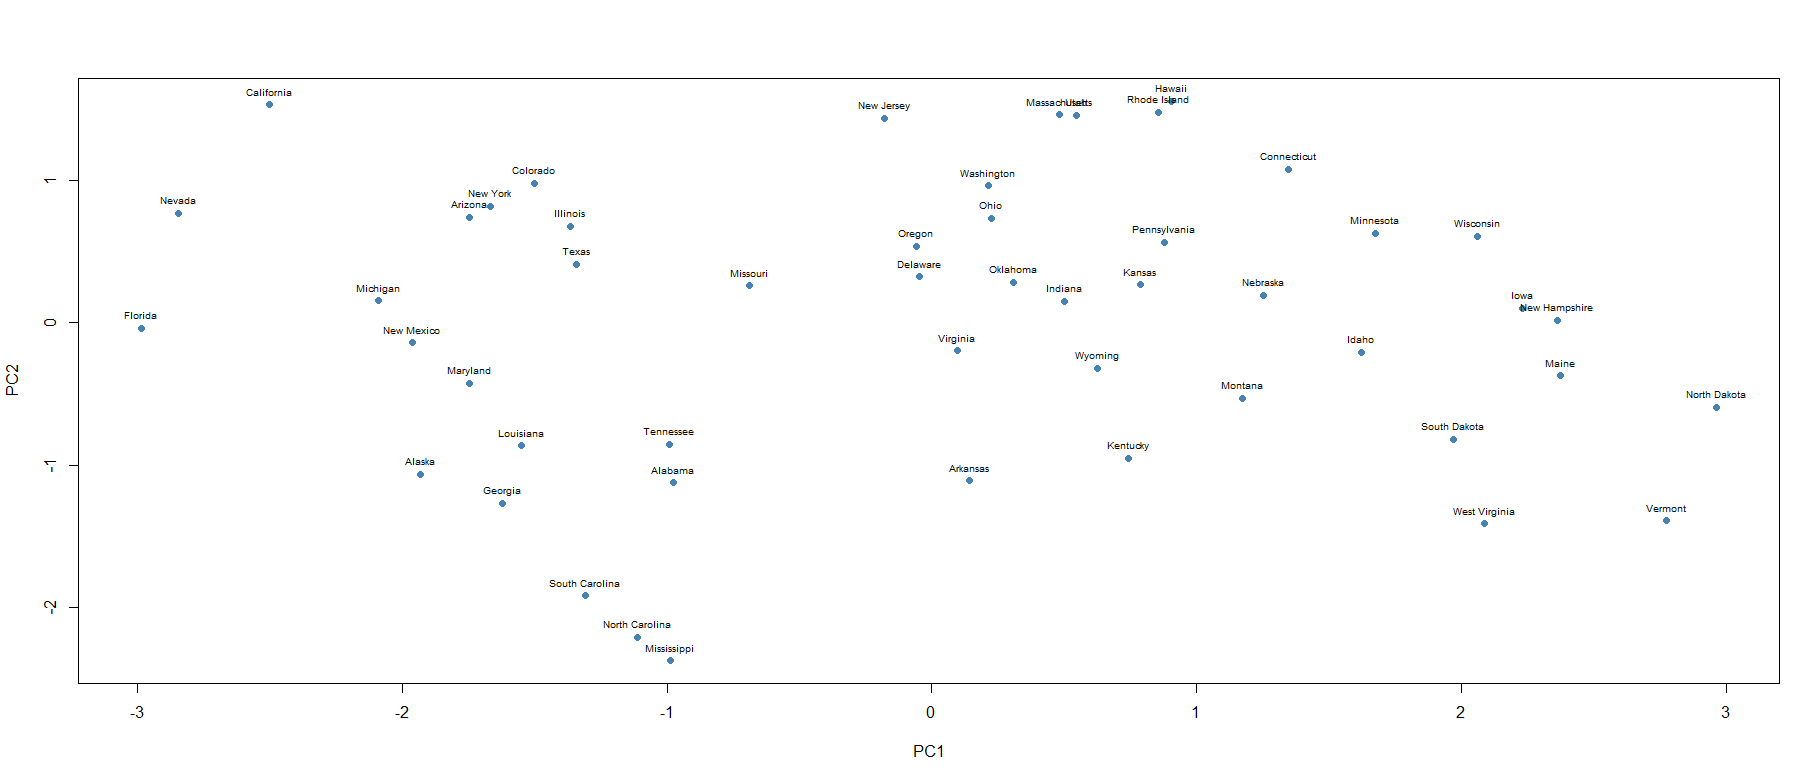
\includegraphics[width=0.9\textwidth]{PC1vsPC2}
\end{center}
    \end{solucion}








    
    \item Interprete la información que representa cada componente
      principal.
  \end{enumerate}

\begin{solucion}

\begin{lstlisting}
summary(pca)
\end{lstlisting}

\begin{lstlisting}
Importance of components:
                          PC1    PC2     PC3     PC4
Standard deviation     1.5749 0.9949 0.59713 0.41645
Proportion of Variance 0.6201 0.2474 0.08914 0.04336
Cumulative Proportion  0.6201 0.8675 0.95664 1.00000
\end{lstlisting}


 Las dos primeras componentes concentran el $86.75\%$ de la varianza total, por lo que basta con analizarlas a ellas \citep{gil_pca_rpubs,serrano_pca_video}.
 
\begin{lstlisting}
pca[["rotation"]]
                PC1        PC2        PC3         PC4
Murder   -0.5358995 -0.4181809  0.3412327  0.64922780
Assault  -0.5831836 -0.1879856  0.2681484 -0.74340748
UrbanPop -0.2781909  0.8728062  0.3780158  0.13387773
Rape     -0.5434321  0.1673186 -0.8177779  0.08902432
\end{lstlisting}

Para el primer componente 1 (62.01\% de la varianza), sus loadings son
      \[
        \text{PC}_1 = -0.536\,\text{Murder}_z -0.583\,\text{Assault}_z
        -0.278\,\text{UrbanPop}_z -0.543\,\text{Rape}_z .
      \]


  Los coeficientes de Murder, Assault y Rape son de magnitud muy similar (entre $-0.54$ y $-0.58$), y considerablemente mayores en valor absoluto que el de UrbanPop ($-0.278$). Por lo tanto, PC1 puede interpretarse como el indicador de criminalidad violenta.

Para el componente 2 (24.74\% de la varianza), sus  loadings son
      \[
        \text{PC}_2 = - 0.418\,\text{Murder}_z  - 0.188\,\text{Assault}_z
        + 0.873\,\text{UrbanPop}_z + 0.167\,\text{Rape}_z .
      \]
      Aquí domina claramente el coeficiente de UrbanPop ($-0.873$), muy por
      encima del resto. Esto indica que PC2 representa principalmente el
      grado de urbanización de cada estado.


    En conclusión, las dos primeras componentes principales resumen, de
      forma casi independiente, dos aspectos distintos de los datos:
      qué tan violento es un estado (PC1) y qué tan urbano es
      (PC2), conservando el $86.75\%$ de la información original en solo dos
      dimensiones.

    
\end{solucion}



  
\end{ejercicio}


% EJERCICIO 6

\begin{ejercicio}[15 puntos]
      Lea el artículo Genes mirror geography within Europe, que se encuentra en
  la carpeta de referencias compartida de Drive.
  \url{https://drive.google.com/drive/u/0/folders/1F-FI1J5PviBc-EPhfLbnE8PSvWnkgeHj}
  Explique de forma resumida de qué se trata el artículo y realice un
  conclusión de cómo el algoritmo de componentes principales es de gran
  utilidad en la reducción de la dimensionalidad.
\end{ejercicio}


\begin{solucion}
Este artículo \cite{novembre2008} estudia qué tanto se parece la variación genética de los europeos a su distribución geográfica. Los autores usaron datos del proyecto POPRES: unos 3.000 individuos genotipados en más de 500.000 SNP (variantes de ADN). Después de aplicar filtros de calidad y de origen, el análisis se hizo con 1.387 individuos y 197.146 SNP.
 
Para resumir toda esa información genética usaron el análisis de componentes principales (PCA), quedándose solo con los dos primeros componentes, PC1 y PC2. Al graficar a los individuos con estos dos ejes, el resultado se parece notablemente a un mapa de Europa: las poblaciones vecinas quedan cerca entre sí y se distinguen zonas como la península ibérica, la itálica y el sureste europeo. Incluso se detecta estructura entre los suizos según su idioma (francés, alemán o italiano).
 
Esta relación también se comprobó de manera numérica: tras rotar los ejes del PCA, el eje genético norte-sur se correlacionó con la latitud ($r^2 = 0{,}77$) y el eje este-oeste con la longitud ($r^2 = 0{,}78$).
 
Además, esta representación reducida sirve para estimar el origen geográfico de una persona. Con un método de asignación basado en regresión sobre PC1 y PC2, el 50\,\% de los individuos quedó a menos de 310 km de su origen reportado y el 90\,\% a menos de 700 km.


\textbf{Conclusión:} Existe una gran utilidad del análisis de componentes principales en la reducción de la dimensionalidad, para este articulo cada individuo tiene casi 200.000 dimensiones (una por SNP), lo que hace imposible visualizarlas o interpretarlas directamente. El PCA transforma esa información en solo dos ejes que conservan la información más importante, en este caso, la estructura geográfica de la población europea.
 
Es notable que PC1 y PC2 explican apenas el $0.30\%$ y el $0.15\%$ de la variación total, y aun así capturan un patrón claro. Esto ocurre porque la señal de ancestría es coherente a lo largo de miles de SNP, mientras que el ruido y la variación individual se reparten en muchas otras direcciones.
 
De esta manera, se puede decir que el PCA facilita la visualización, la interpretación y el análisis de datos de alta dimensionalidad, y conserva los patrones relevantes de los datos originales \citep{gil_pca_rpubs,serrano_pca_video}. Este artículo lo demuestra al convertir un conjunto de datos genéticos muy complejo en una representación bidimensional comprensible, que permite identificar relaciones difíciles de observar de otra forma.

\end{solucion}



\bibliographystyle{unsrtnat}
\bibliography{referencias}

\end{document}
